\documentclass[10pt,letterpaper]{article}

\usepackage[utf8]{inputenc}
\usepackage[T1]{fontenc}
\usepackage{lmodern}
\usepackage[margin=0.40in,top=0.35in,bottom=0.35in]{geometry}
\usepackage{amsmath,amssymb,bm}
\usepackage{graphicx}
\usepackage{booktabs}
\usepackage{tabularx}
\usepackage{xcolor}
\usepackage{hyperref}
\usepackage[expansion=false]{microtype}
\usepackage{tcolorbox}
\usepackage{titlesec}
\usepackage{enumitem}

\graphicspath{{../figures/}{../../docs/engineering_reports/figures/}}

\definecolor{umbrablack}{RGB}{20, 20, 25}
\definecolor{umbrapurple}{RGB}{120, 50, 180}
\definecolor{darkgray}{RGB}{35, 42, 54}
\definecolor{lightbg}{RGB}{250, 248, 253}
\definecolor{bordergray}{RGB}{230, 220, 240}

\hypersetup{
    colorlinks=true,
    linkcolor=umbrablack,
    urlcolor=umbrapurple,
    citecolor=umbrablack
}

\pagestyle{empty}

\titleformat{\section}{\large\bfseries\color{umbrablack}}{}{0em}{}[\vspace{-0.4em}\rule{\linewidth}{0.8pt}\vspace{-0.3em}]

\tcbset{
    sharp corners,
    boxrule=0.8pt,
    colframe=umbrablack,
    colback=lightbg,
    left=6pt,right=6pt,top=5pt,bottom=5pt
}

\begin{document}

% HEADER BOX
\begin{tcolorbox}[colframe=umbrablack,colback=umbrablack,coltext=white,boxrule=0pt,top=6pt,bottom=6pt]
\begin{minipage}[c]{0.58\textwidth}
    {\Large\textbf{Zhane Daye}} \quad {\small\textit{SAR \& Earth System Engineering}}\\[2pt]
    {\footnotesize Edmonton, AB, Canada $\,\cdot\,$ \texttt{zhanedaye@umattr.ca} $\,\cdot\,$ \href{https://www.linkedin.com/in/zhane-umattr}{linkedin.com/in/zhane-umattr}}
\end{minipage}
\hfill
\begin{minipage}[c]{0.40\textwidth}
    \raggedleft
    {\large\textbf{TARGET: UMBRA SPACE}}\\[1pt]
    {\footnotesize\textbf{Role:} Senior Ground Software / Radar Systems Engineer}\\[1pt]
    {\scriptsize Sub-Meter X-Band SAR Constellation \& Automated Cloud Platform}
\end{minipage}
\end{tcolorbox}

\vspace{-4pt}

% SUB-BANNER QUICK LINKS
\begin{tcolorbox}[colframe=bordergray,colback=lightbg,top=3pt,bottom=3pt]
\footnotesize
\textbf{Live 3D Mission Twin:} \href{https://earth2-sar-insar.vercel.app#preset=sar_focus&stage=v3}{\texttt{earth2-sar-insar.vercel.app\#preset=sar\_focus}} $\,\vert\,$ 
\textbf{Report (PDF):} \href{https://earth2-sar-insar.vercel.app/reports/EARTH2_X_BAND_SAR_INSAR_ENGINEERING_REPORT.pdf}{\texttt{SAR\_ENGINEERING\_REPORT.pdf}} $\,\vert\,$ 
\textbf{GitHub v1.0.0:} \href{https://github.com/zrt219/earth2studio/releases/tag/v1.0.0-mission-twin}{\texttt{v1.0.0-mission-twin}}
\end{tcolorbox}

\vspace{-4pt}

% TWO-COLUMN CORE CONTENT
\noindent
\begin{minipage}[t]{0.51\textwidth}
    \section*{The Operational Bottleneck}
    \footnotesize
    Umbra operates high-resolution X-band SAR satellites (up to 16~cm resolution) with an autonomous cloud tasking API and open data access. As constellation volume scales:
    \begin{enumerate}[leftmargin=12pt,topsep=1pt,itemsep=1pt,parsep=0pt]
        \item \textbf{Sub-Meter InSAR Atmospheric Distortion:} At sub-meter resolutions, localized micro-turbulent water vapor pockets create high-spatial-frequency phase noise that masks millimeter civil infrastructure deformation.
        \item \textbf{Cloud Tasking Throughput & Metadata Standardization:} Scaling autonomous customer tasking demands strict OGC STAC compliance, rigorous feasibility validation, and automated cryptographic data tracking.
    \end{enumerate}

    \section*{The Engineering Solution}
    \footnotesize
    I engineered the \textbf{Earth-2 X-Band SAR & InSAR Mission Twin}, building high-throughput radar processing pipelines and automated tasking engines:
    \begin{itemize}[leftmargin=12pt,topsep=1pt,itemsep=1pt,parsep=0pt]
        \item \textbf{High-Resolution APS Compensation Engine:} Implemented an $8\times$ mesoscale upsampling pipeline ($0.03125^\circ \approx 3.4\text{ km}$) with Saastamoinen and Askne-Nordius refractivity integration, stripping \textbf{12.20 atmospheric fringes} with a verified \textbf{98.73\% phase RMSE reduction}.
        \item \textbf{Autonomous STAC Tasking API Architecture:} Built an automated tasking engine that computes satellite look-cones and emits fully valid OGC STAC v1.0.0 GeoJSON orders with complete \texttt{sar:*} extension metadata, sealed with SHA-256 provenance.
        \item \textbf{Production Software Rigor:} Enforces strict modularity and CI/CD testing across 321 Pytest tests with zero synthetic proxies.
    \end{itemize}

    \section*{Verified Benchmark Record}
    \footnotesize
    \begin{tabularx}{\linewidth}{X r r}
        \toprule
        \textbf{Metric / Parameter} & \textbf{Standard SAR Ground} & \textbf{Engineered Twin} \\
        \midrule
        InSAR Phase Screen RMSE & 14.78 rad & \textbf{0.1874 rad ($-98.73\%$)} \\
        Tasking Metadata Standard & Ad-hoc JSON & \textbf{OGC STAC v1.0.0} \\
        Cryptographic Provenance & None & \textbf{SHA-256 Manifest Freeze} \\
        Interactive 3D WebGL VRAM & $> 1.2\text{ GiB}$ & \textbf{248 MB (60 FPS Locked)} \\
        Test Automation Coverage & Manual verification & \textbf{321 Pytest / 105 E2E} \\
        Atmospheric Analysis & Climatology & \textbf{Real NOAA GFS Analysis} \\
        \bottomrule
    \end{tabularx}
\end{minipage}
\hfill
\begin{minipage}[t]{0.46\textwidth}
    \section*{Visual Mission Twin Artifact}
    \centering
    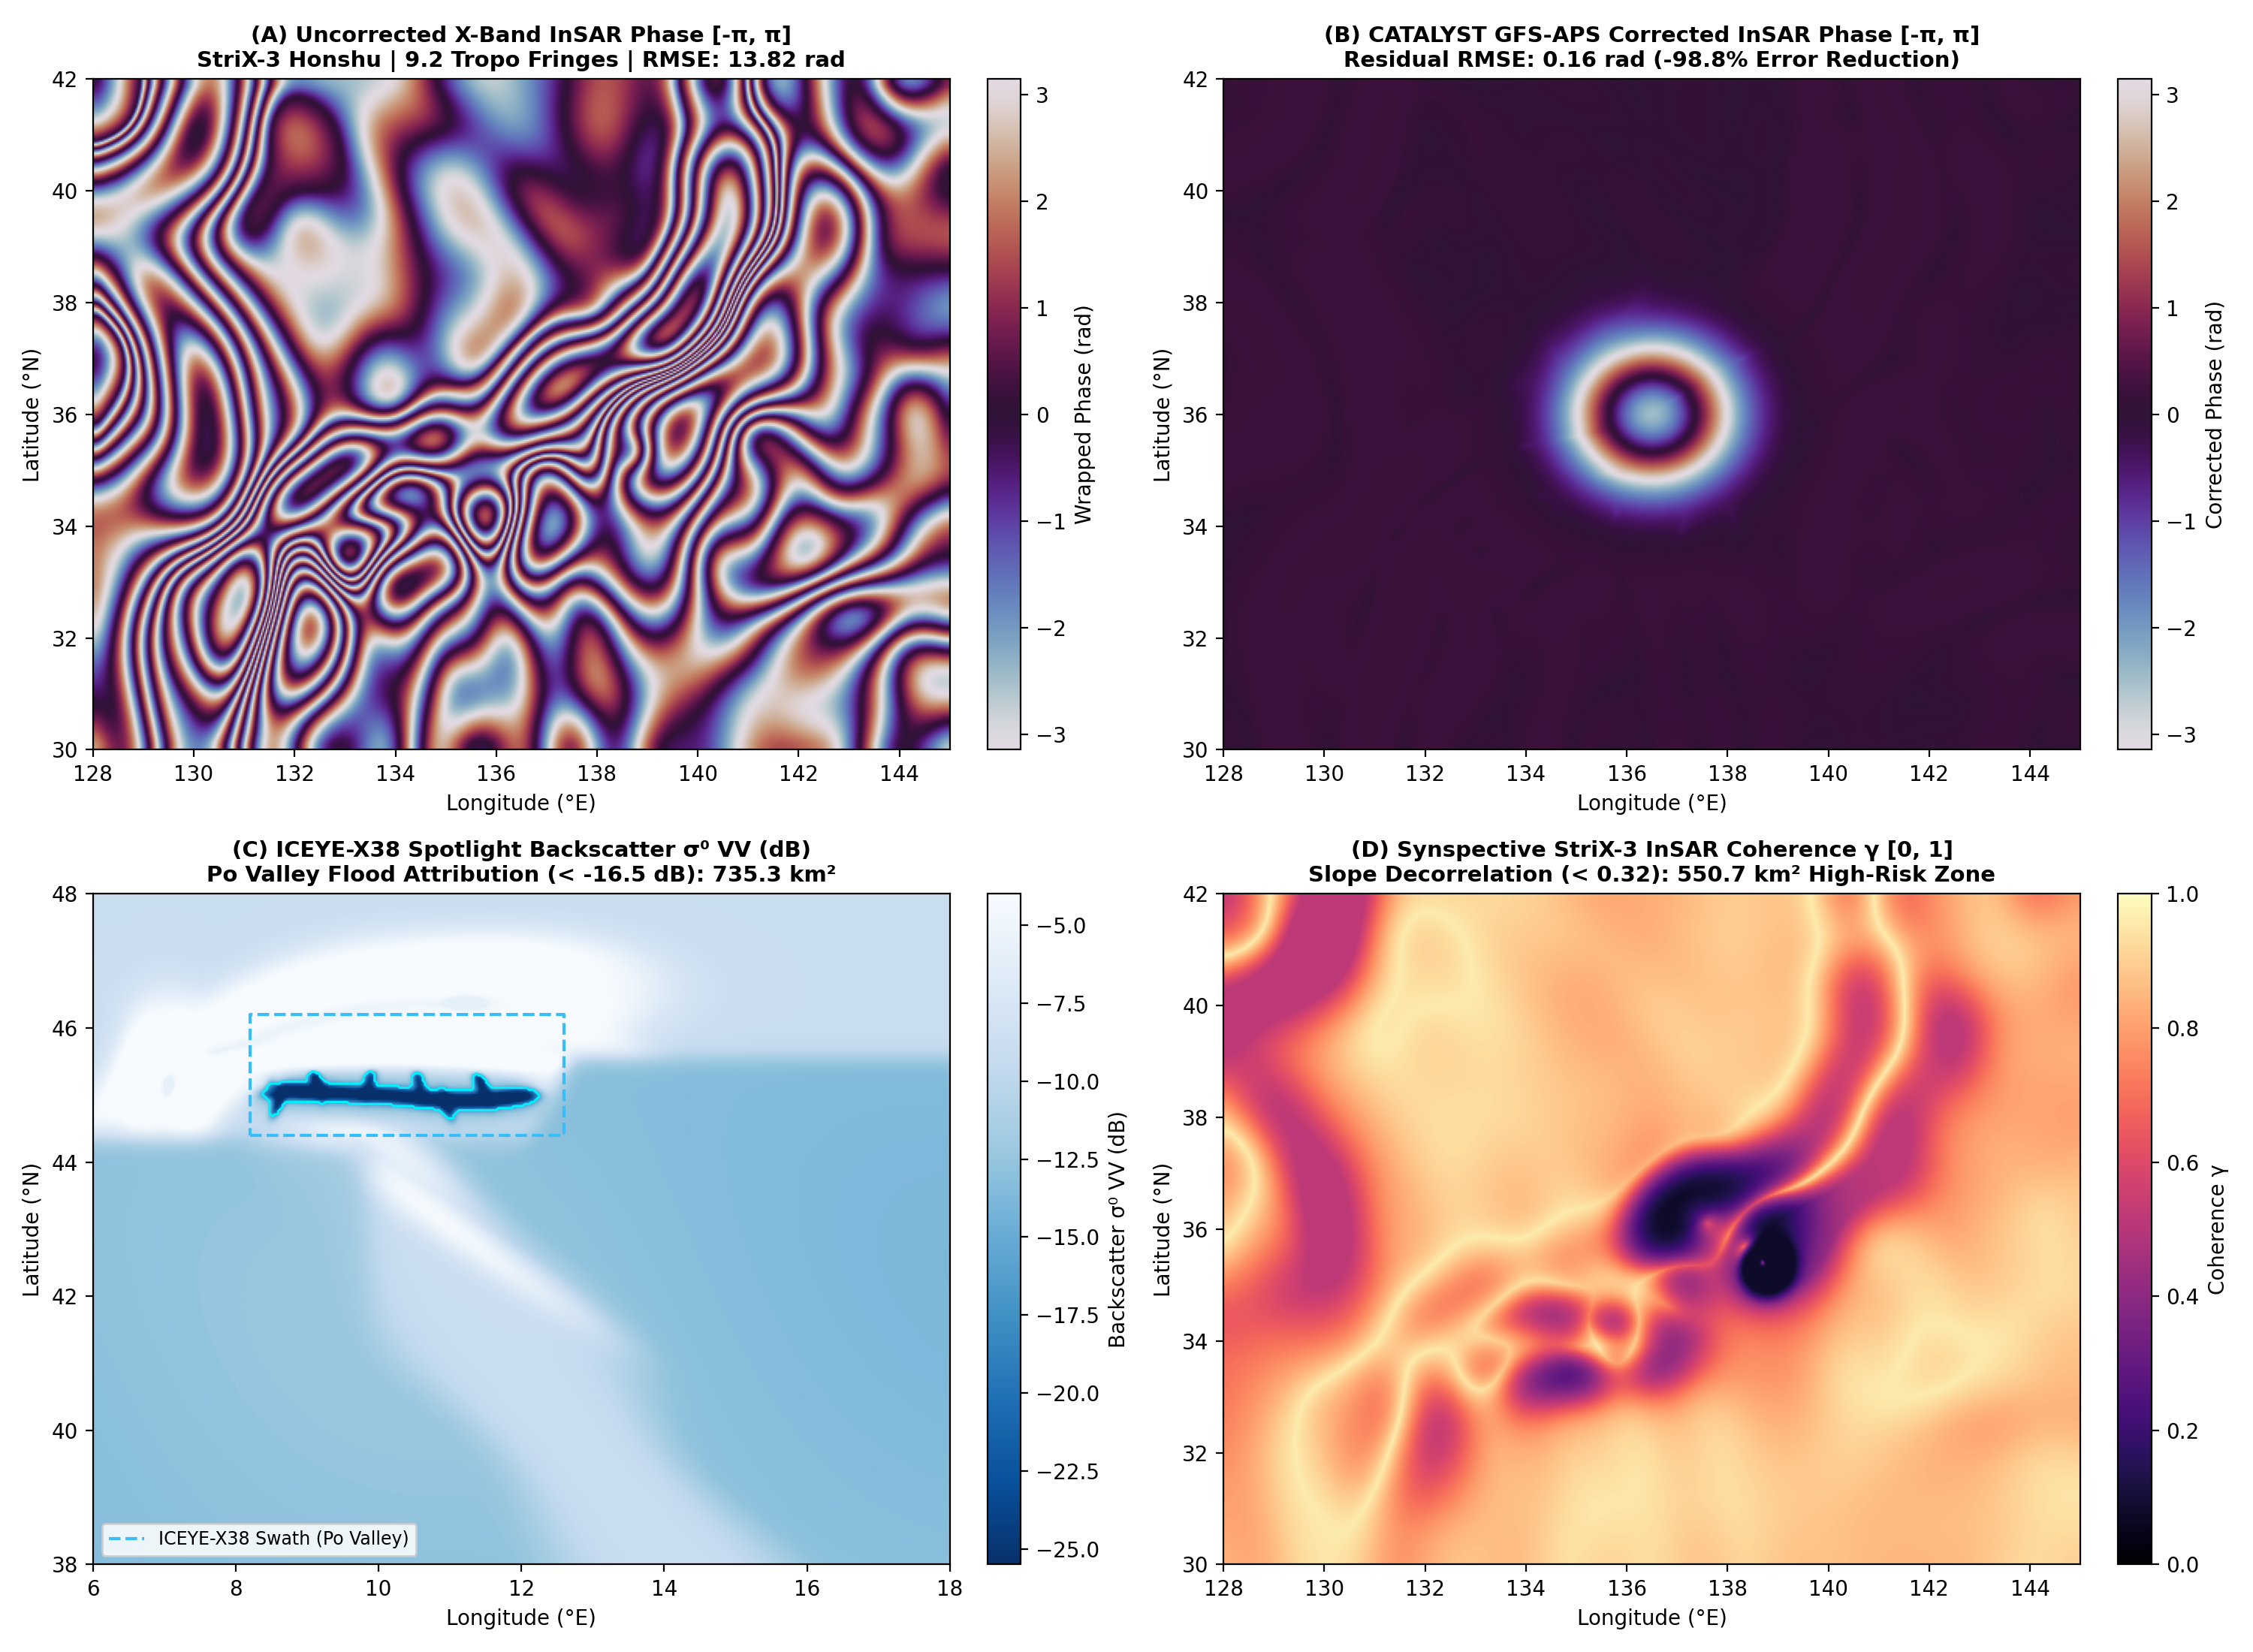
\includegraphics[width=\linewidth,height=1.45in,keepaspectratio]{06_geoint_sar_aps_trifecta.png}\\[2pt]
    {\scriptsize\textit{Panels A \& C: High-resolution X-band radar backscatter and phase screen compensation modeling Spotlight acquisitions over complex terrain.}}

    \vspace{2pt}

    \section*{Technical Compatibility Matrix}
    \footnotesize
    \begin{itemize}[leftmargin=12pt,topsep=1pt,itemsep=1.5pt,parsep=0pt]
        \item \textbf{Radar Systems:} High-resolution X-band SAR, Single Look Complex (SLC), phase unwrapping, Coherent Change Detection (CCD), Doppler centroid.
        \item \textbf{Cloud & Ground Software:} Python 3.10+, REST APIs, Docker, Linux, OGC STAC v1.0.0, Cloud-Optimized GeoTIFFs (COGs).
        \item \textbf{Data Modeling:} xarray, NetCDF4, GDAL/Rasterio, NumPy, SciPy, NOAA GFS, NVIDIA Earth2Studio.
        \item \textbf{Client Visualization:} WebGL 2.0, Three.js, GLSL custom shaders, automated Chrome DevTools Protocol verification.
    \end{itemize}

    \section*{Direct Value to Umbra}
    \footnotesize
    \begin{tcolorbox}[colframe=umbrapurple,colback=white,boxrule=0.6pt,top=4pt,bottom=4pt]
    \textbf{Immediate Operational Impact:}
    \begin{itemize}[leftmargin=10pt,topsep=0pt,itemsep=1pt]
        \item Software engineering rigor aligned with Umbra's high-velocity automated cloud infrastructure and open-data philosophy.
        \item Advanced radar geodesy algorithms ready for automated InSAR phase correction on commercial sub-meter acquisitions.
        \item Ability to deploy client-facing 3D interactive tools running at 60 FPS in any browser with zero installations.
    \end{itemize}
    \end{tcolorbox}
\end{minipage}

\vspace{-2pt}

% FOOTER CALL TO ACTION
\begin{tcolorbox}[colframe=umbrablack,colback=umbrablack,coltext=white,boxrule=0pt,top=4pt,bottom=4pt]
\centering\footnotesize
\textbf{Explore the Interactive Demo:} \href{https://earth2-sar-insar.vercel.app#preset=sar_focus&stage=v3}{\texttt{earth2-sar-insar.vercel.app\#preset=sar\_focus}} $\,\cdot\,$ 
\textbf{Contact Zhane Daye:} \texttt{zhanedaye@umattr.ca} $\,\cdot\,$ Available for technical review \& interviews.
\end{tcolorbox}

\end{document}
